\documentclass[10pt]{beamer}
\usepackage{ctex,hyperref}
\usepackage{amsmath,amssymb,booktabs,graphicx,xcolor,multicol,tabularx,array}
\usepackage{tikz}
\usetikzlibrary{positioning,arrows.meta}
\usepackage{pgfplots}
\pgfplotsset{compat=1.18}

\usepackage{RenminUniv}

\setsansfont{Arial}
\setCJKmainfont{KaiTi}
\setCJKsansfont{KaiTi}

\title{生成式模型用于 KiTS23 肾脏肿瘤分割}
\subtitle{判别式基线与条件生成式分割模型对比}
\author[刘嘉俊 / 安昊宇]{\texorpdfstring{刘嘉俊 \quad 2023200431 \\ 安昊宇 \quad 2024201650}{刘嘉俊 2023200431 / 安昊宇 2024201650}}
\institute[高瓴人工智能学院]{中国人民大学高瓴人工智能学院}
\date{2026 年 6 月}

\setbeamertemplate{navigation symbols}{}
\setbeamerfont{title}{family=\sffamily,series=\bfseries,size=\Large}
\setbeamerfont{subtitle}{family=\sffamily,size=\small}
\setbeamerfont{frametitle}{family=\sffamily,series=\bfseries,size=\large}
\setbeamerfont{block title}{family=\sffamily,series=\bfseries}
\setbeamerfont{normal text}{size=\footnotesize}
\setbeamerfont{block body}{size=\footnotesize}

\definecolor{ruc}{RGB}{151,31,48}
\definecolor{deepgreen}{RGB}{0,122,104}
\definecolor{ink}{RGB}{34,34,34}
\definecolor{softgray}{RGB}{244,246,250}
\definecolor{amber}{RGB}{214,126,28}

\newcommand{\model}[1]{\textsf{#1}}
\newcommand{\codepath}[1]{\texttt{\scriptsize\detokenize{#1}}}
\newcommand{\sourcefoot}[1]{\vspace{0.25em}{\tiny\color{gray!70}#1}}
\newcommand{\metricup}[1]{\textcolor{deepgreen}{\textbf{#1}}}
\newcommand{\metricbad}[1]{\textcolor{ruc}{\textbf{#1}}}
\newcommand{\takeaway}[1]{\vspace{0.2em}{\footnotesize\textcolor{ruc}{\textbf{结论：}}#1}}

\begin{document}

\begin{frame}
  \titlepage
  \begin{figure}
    \centering
    
\includegraphics[width=0.28\linewidth]{pic/Renmin_Univ_Logo.eps}
  \end{figure}
\end{frame}


\begin{frame}{目录}
  \tableofcontents[sectionstyle=show,subsectionstyle=show/shaded/hide]
\end{frame}

\section{任务与数据}

\begin{frame}{任务定义：KiTS23 四类分割}
  \begin{columns}[T]
    \column{0.56\textwidth}
      \begin{block}{输入与输出}
        给定腹部 CT axial slice $x\in\mathbb{R}^{C\times256\times256}$，预测逐像素标签：
        \[
          y_i\in\{0,1,2,3\}
          =\{\text{背景},\text{肾脏},\text{肿瘤},\text{囊肿}\}.
        \]
        评价时分别计算 kidney、tumor、cyst 的 Dice / IoU，并报告三类前景平均值。
      \end{block}
      \begin{alertblock}{任务难点}
        肾脏区域较大且形态稳定；肿瘤和囊肿面积小、类别不均衡强，且 2D 切片缺少跨层连续性，因此小病灶最容易漏检。
      \end{alertblock}

    \column{0.40\textwidth}
      \begin{block}{数据划分}
        \centering
        \setlength{\tabcolsep}{3pt}
        \begin{tabular}{lrrr}
          \toprule
          划分 & 病例 & 切片 & 前景切片 \\
          \midrule
          训练 & 70 & 6950 & 5585 \\
          验证 & 15 & 1624 & 1323 \\
          测试 & 15 & 1151 & 901 \\
          \bottomrule
        \end{tabular}
      \end{block}
      \begin{exampleblock}{预处理}
        HU window $c=40,w=400$；归一化到 $[0,1]$；resize 到 $256\times256$；按病例划分防止数据泄漏。
      \end{exampleblock}
  \end{columns}
\end{frame}

\begin{frame}{数据处理流程}
  \begin{columns}[T]
    \column{0.54\textwidth}
      \begin{block}{从 3D CT 到 2D axial slice}
        \begin{itemize}
          \item 从 NIfTI 文件读取 CT 体数据和体素级标注；
          \item 保留前景切片及其上下文，稀疏保留纯背景切片；
          \item 生成训练、验证、测试 CSV，保证 patient-level split。
        \end{itemize}
      \end{block}
    \column{0.42\textwidth}
      \begin{exampleblock}{输入设置}
        主实验使用 2D 单切片；扩展实验使用 2.5D 输入，即相邻三张切片作为 3 通道。
      \end{exampleblock}
  \end{columns}
\end{frame}

\section{方法设计}

\begin{frame}{整体实验设计}
  \begin{columns}[T]
    \column{0.48\textwidth}
      \begin{exampleblock}{判别式分割}
        直接学习从 CT 到 mask 的映射：
        \[
          \hat y=f_\theta(x).
        \]
        本项目使用 U-Net、SegResNet 和 2.5D U-Net 作为基线。
      \end{exampleblock}
    \column{0.48\textwidth}
      \begin{alertblock}{生成式分割}
        将 mask 看作随机变量，学习条件分布：
        \[
          p_\theta(y\mid x).
        \]
        本项目实现 conditional VAE 与 conditional diffusion。
      \end{alertblock}
  \end{columns}
  \vspace{0.5em}
  \begin{block}{统一评价}
    所有模型在同一 axial test split 上评估，报告 Mean Dice、Mean IoU、各类别 Dice 和单张图像推理时间。
  \end{block}
\end{frame}

\section{判别式模型}

\begin{frame}{判别式基线：U-Net、SegResNet 与 2.5D 输入}
  \begin{columns}[T]
    \column{0.52\textwidth}
      \begin{block}{模型思路}
        \begin{itemize}
          \item \model{U-Net}：编码器-解码器结构，通过 skip connection 保留空间细节；
          \item \model{SegResNet}：残差块增强特征表达能力；
          \item \model{2.5D U-Net}：将相邻切片拼接为多通道输入，引入局部 3D 上下文。
        \end{itemize}
      \end{block}
    \column{0.44\textwidth}
      \begin{exampleblock}{损失函数}
        使用 DiceCE 同时优化像素分类和区域重叠：
        \[
          \mathcal{L}
          =
          \mathcal{L}_{\mathrm{CE}}
          +
          \mathcal{L}_{\mathrm{Dice}}.
        \]
      \end{exampleblock}
      \sourcefoot{主要代码：\codepath{src/models/unet_baseline.py}, \codepath{src/models/segresnet_baseline.py}}
  \end{columns}
\end{frame}

\begin{frame}{判别式基线结果}
  \begin{block}{测试集结果}
    \centering
    \setlength{\tabcolsep}{4pt}
    \begin{tabular}{lrrrrr}
      \toprule
      模型 & Mean Dice & Kidney & Tumor & Cyst & ms/img \\
      \midrule
      U-Net 2D & 0.570 & 0.912 & 0.623 & 0.177 & 2.57 \\
      SegResNet 2D & 0.572 & 0.914 & 0.621 & 0.181 & 4.46 \\
      U-Net 2.5D & \metricup{0.623} & 0.921 & 0.707 & 0.242 & 2.49 \\
      \bottomrule
    \end{tabular}
  \end{block}
  \begin{alertblock}{观察}
    2.5D U-Net 明显优于 2D U-Net，说明相邻切片上下文对肿瘤和囊肿等小结构有帮助。
  \end{alertblock}
\end{frame}

\section{生成式模型}

\begin{frame}{生成式分割建模}
  \begin{columns}[T]
    \column{0.52\textwidth}
      \begin{block}{从确定性预测到条件分布}
        判别式模型通常输出一个确定 mask。生成式模型将 mask 视为条件随机变量：
        \[
          y\sim p_\theta(y\mid x).
        \]
        这样可以通过采样得到多个候选结果，并进一步分析模型不确定性。
      \end{block}
    \column{0.44\textwidth}
      \begin{exampleblock}{本项目生成式模型}
        \begin{itemize}
          \item conditional VAE；
          \item conditional diffusion；
        \end{itemize}
      \end{exampleblock}
  \end{columns}
  \takeaway{生成式模型的目标不是只追求单点 Dice，而是同时提供生成过程和不确定性分析。}
\end{frame}

\begin{frame}{条件 VAE：潜变量生成分割掩码}
  \begin{columns}[T]
    \column{0.55\textwidth}
      \begin{block}{模型形式}
        给定 CT 图像 $x$ 和真实 mask $y$，编码器近似后验：
        \[
          q_\phi(z\mid x,y),
        \]
        解码器根据图像条件和潜变量生成 mask：
        \[
          \hat y\sim p_\theta(y\mid x,z).
        \]
      \end{block}
      \begin{exampleblock}{训练目标}
        \[
          \mathcal{L}_{\mathrm{cVAE}}
          =
          \mathcal{L}_{\mathrm{DiceCE}}(\hat y,y)
          +\beta D_{\mathrm{KL}}(q_\phi(z\mid x,y)\|p(z)).
        \]
      \end{exampleblock}
    \column{0.41\textwidth}
      \centering
      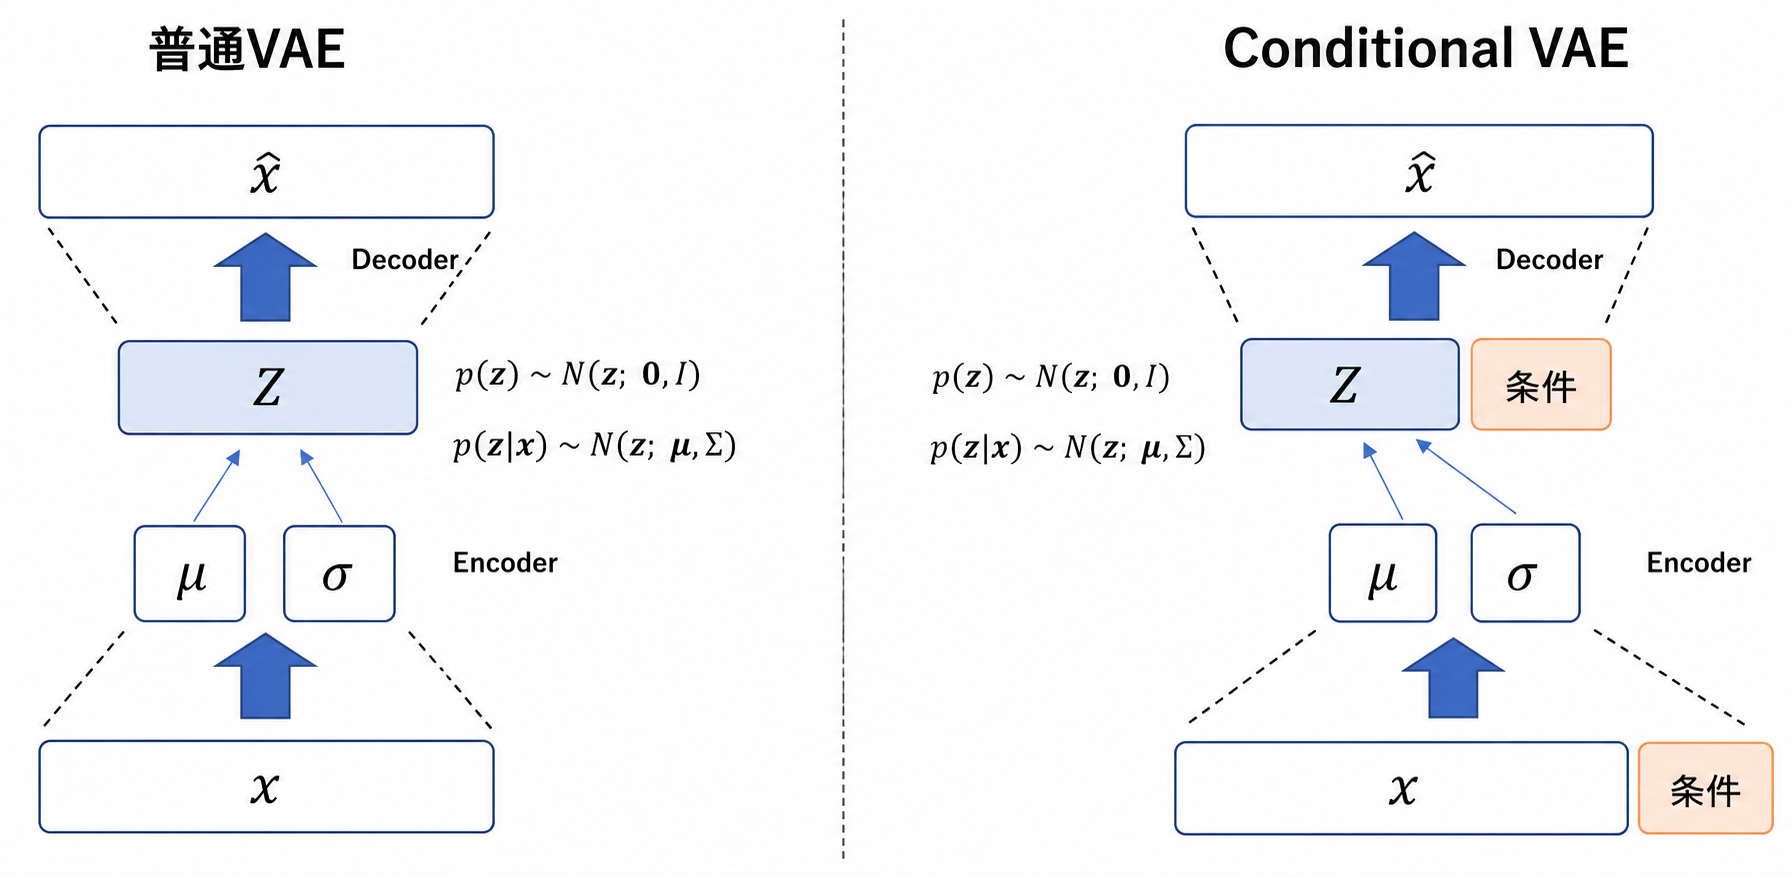
\includegraphics[width=0.92\textwidth]{assets/vae_cvae_diagram.png}
      \sourcefoot{cVAE 作为轻量生成式基线。}
      \begin{alertblock}{测试阶段}
        测试时真实 mask 不可见，只能从先验生成，因此 cVAE 对小目标更不稳定。
      \end{alertblock}
  \end{columns}
\end{frame}

\begin{frame}{条件扩散模型：从 noisy mask 到 clean mask}
  \begin{block}{扩散前向过程}
    对真实 one-hot mask $m_0$ 加噪：
    \[
      m_t=\sqrt{\bar{\alpha}_t}m_0+\sqrt{1-\bar{\alpha}_t}\epsilon,\quad
      \epsilon\sim\mathcal{N}(0,I).
    \]
  \end{block}
  \begin{columns}[T]
    \column{0.48\textwidth}
      \begin{exampleblock}{条件去噪网络}
        网络输入 CT 图像 $x$、加噪 mask $m_t$ 和时间步 $t$，输出对 clean mask 的估计。
      \end{exampleblock}
    \column{0.48\textwidth}
      \begin{alertblock}{采样阶段}
        推理时从随机 mask 出发，用 DDIM 逐步更新，最终通过 argmax 得到四类分割结果。
      \end{alertblock}
  \end{columns}
  \centering
  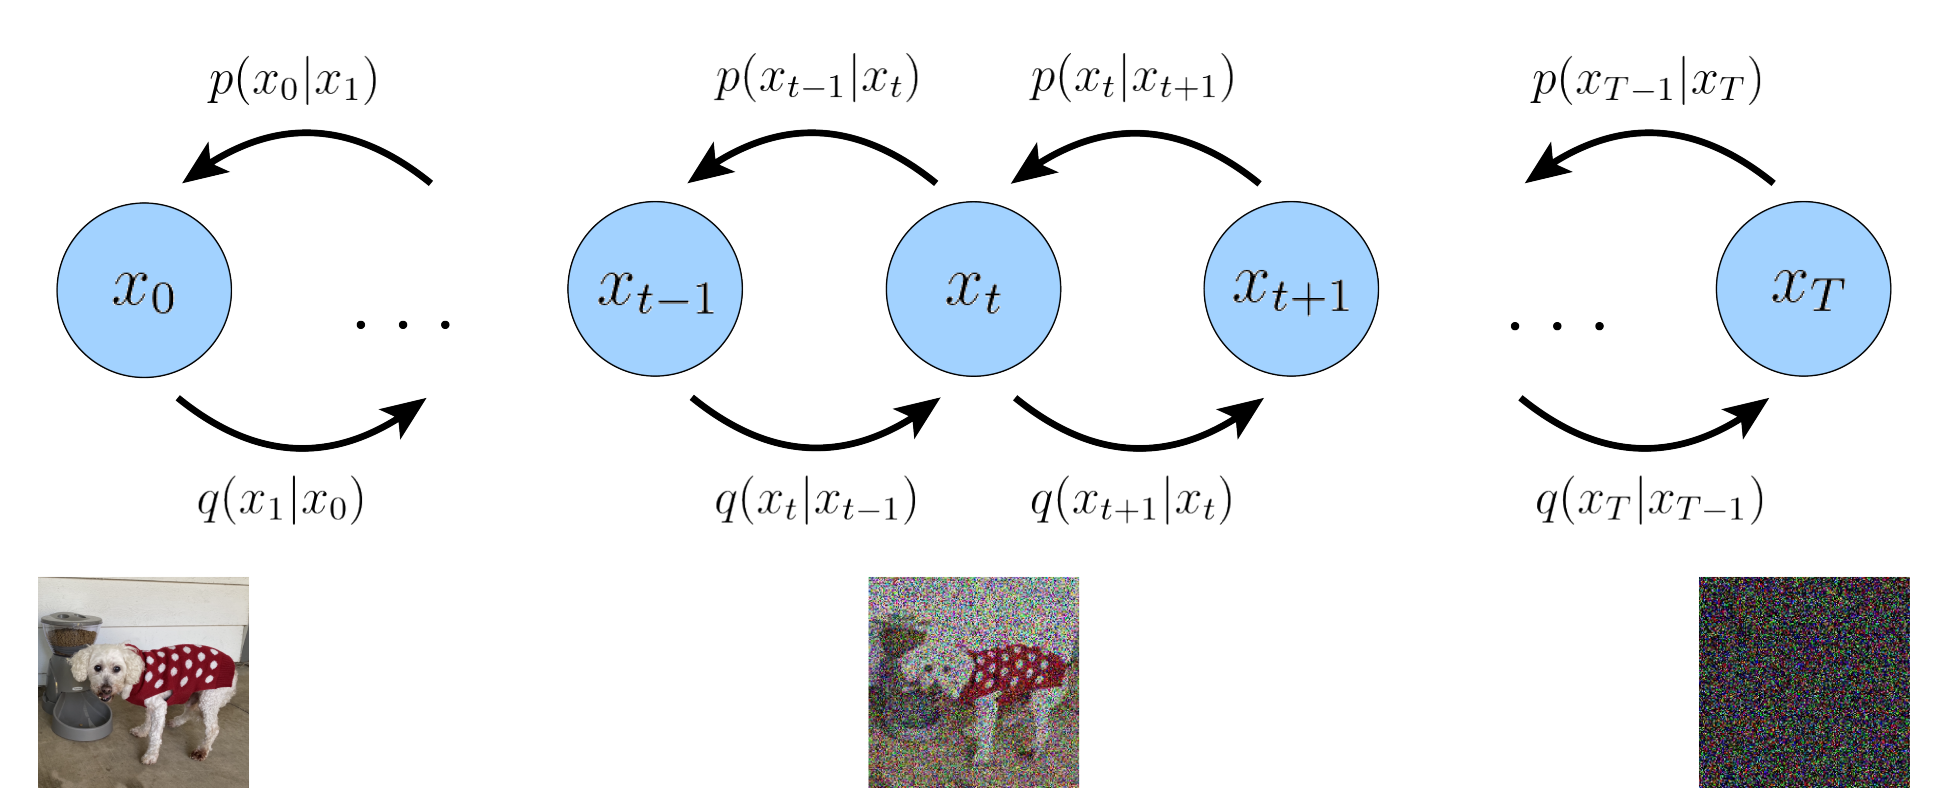
\includegraphics[width=0.55\textwidth]{assets/ddpm_ddim_diagram.png}
\end{frame}

\begin{frame}{x0 Diffusion：使生成目标对齐分割指标}
  \begin{columns}[T]
    \column{0.55\textwidth}
      \begin{block}{直接预测 clean mask}
        本项目采用 x0 形式，让网络直接输出 clean mask logits：
        \[
          \hat m_0=f_\theta(x,m_t,t).
        \]
        训练目标为：
        \[
          \mathcal{L}_{x0}
          =
          \mathcal{L}_{\mathrm{DiceCE}}(\hat m_0,m_0)
          +0.2\|\mathrm{softmax}(\hat m_0)-m_0\|_2^2.
        \]
      \end{block}
    \column{0.41\textwidth}
      \begin{exampleblock}{设计动机}
        医学分割关注语义区域重叠。直接预测 clean mask 可以让训练信号更接近 Dice / IoU 等分割指标。
      \end{exampleblock}
      \begin{block}{主要设置}
        \centering
        \setlength{\tabcolsep}{4pt}
        \begin{tabular}{lr}
          \toprule
          项目 & 设置 \\
          \midrule
          epoch & 80 \\
          batch size & 16 \\
          learning rate & $10^{-4}$ \\
          验证采样步数 & 5 \\
          \bottomrule
        \end{tabular}
      \end{block}
  \end{columns}
\end{frame}

\begin{frame}{条件 U-Net 去噪网络}
  \begin{columns}[T]
    \column{0.52\textwidth}
      \begin{block}{网络输入}
        \codepath{src/models/diffusion_unet.py}\\[2pt]
        stem 输入为 CT 图像和 noisy mask 的拼接：
        \[
          [x,m_t]\in\mathbb{R}^{(C+4)\times256\times256}.
        \]
        其中 2D 实验 $C=1$，2.5D 扩展实验 $C=3$。
      \end{block}
      \begin{exampleblock}{时间步编码}
        每个 residual block 接收 sinusoidal timestep embedding，用于区分不同噪声水平。
      \end{exampleblock}
    \column{0.44\textwidth}
      \centering
      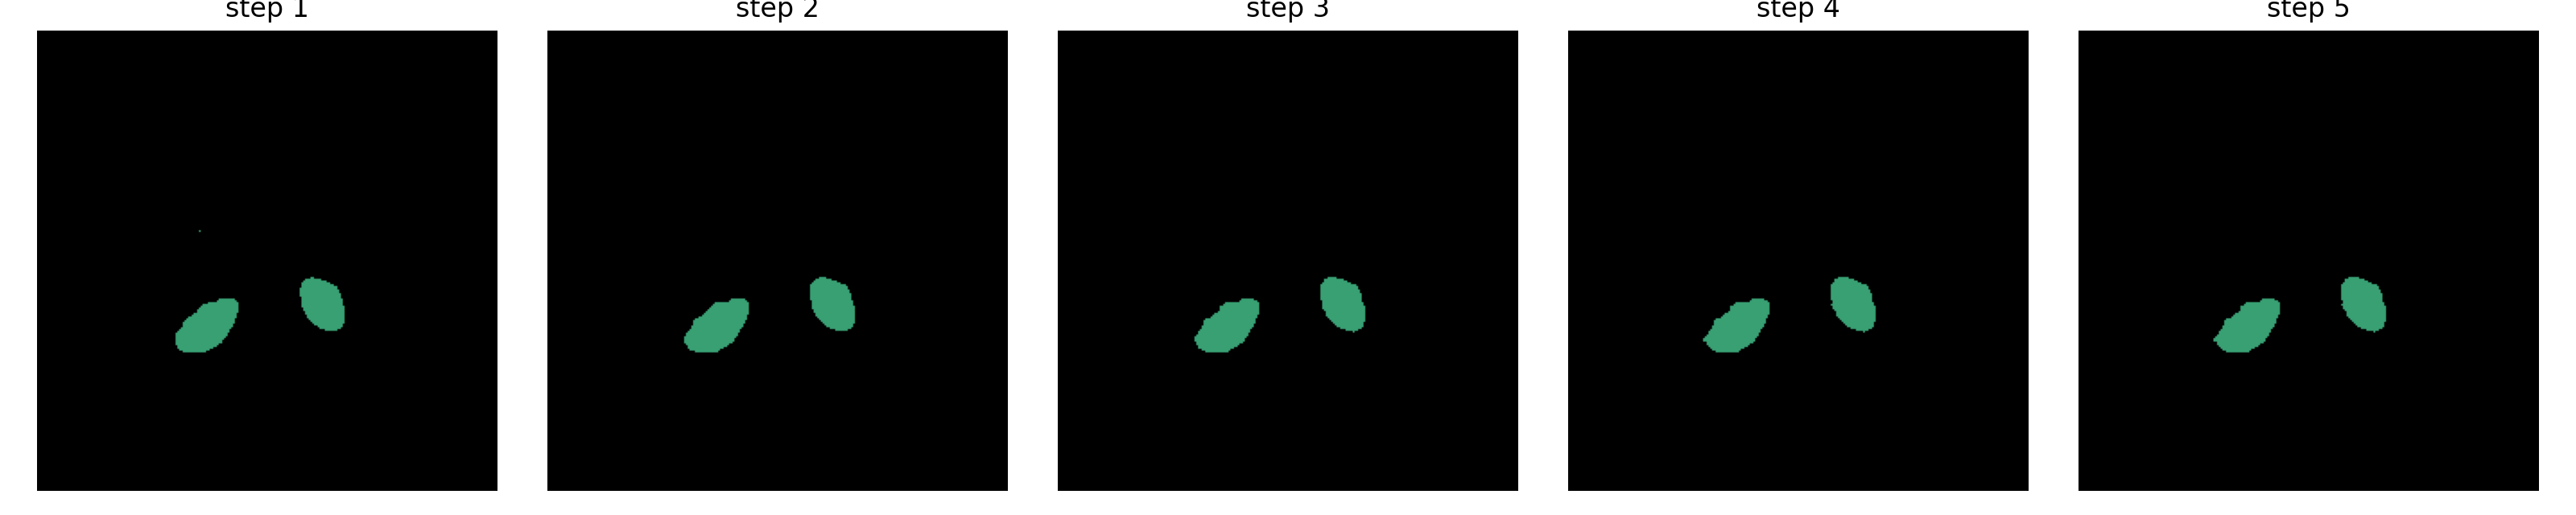
\includegraphics[width=\textwidth]{assets/axial_diffusion_denoising.png}
      \sourcefoot{x0 diffusion 的 5 步去噪轨迹。}
  \end{columns}
\end{frame}

\section{实验与结果}

\begin{frame}{实验设置}
  \begin{columns}[T]
    \column{0.48\textwidth}
      \begin{block}{训练设置}
        \centering
        \setlength{\tabcolsep}{3pt}
        \begin{tabular}{lccc}
          \toprule
          模型 & Epoch & BS & LR \\
          \midrule
          U-Net / SegResNet & 100 & 32 & $2\times10^{-4}$ \\
          cVAE & 100 & 32 & $2\times10^{-4}$ \\
          x0 Diffusion & 80 & 16 & $1\times10^{-4}$ \\
          \bottomrule
        \end{tabular}
      \end{block}
    \column{0.48\textwidth}
      \begin{exampleblock}{评价指标}
        \begin{itemize}
          \item Mean Dice / Mean IoU；
          \item kidney、tumor、cyst 各类别 Dice；
          \item 单张切片推理时间 ms/image；
          \item diffusion 额外比较采样步数。
        \end{itemize}
      \end{exampleblock}
  \end{columns}
  \begin{alertblock}{模型选择}
    所有模型均按验证集 Mean Dice 保存 best checkpoint，再在固定测试集上汇报结果。
  \end{alertblock}
\end{frame}

\begin{frame}{训练曲线}
  \begin{columns}[T]
    \column{0.48\textwidth}
      \centering
      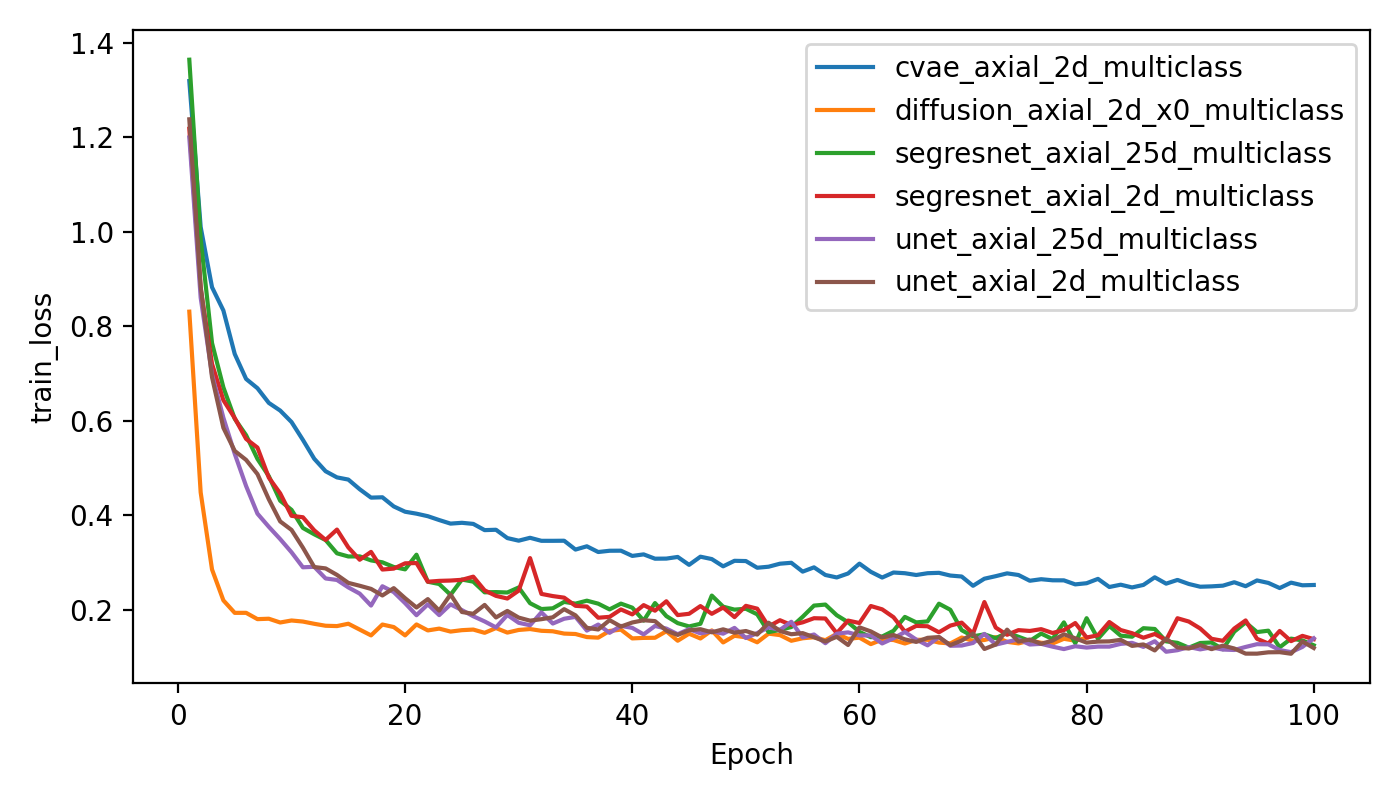
\includegraphics[width=\textwidth]{assets/axial_train_loss.png}
      \sourcefoot{训练损失}
    \column{0.48\textwidth}
      \centering
      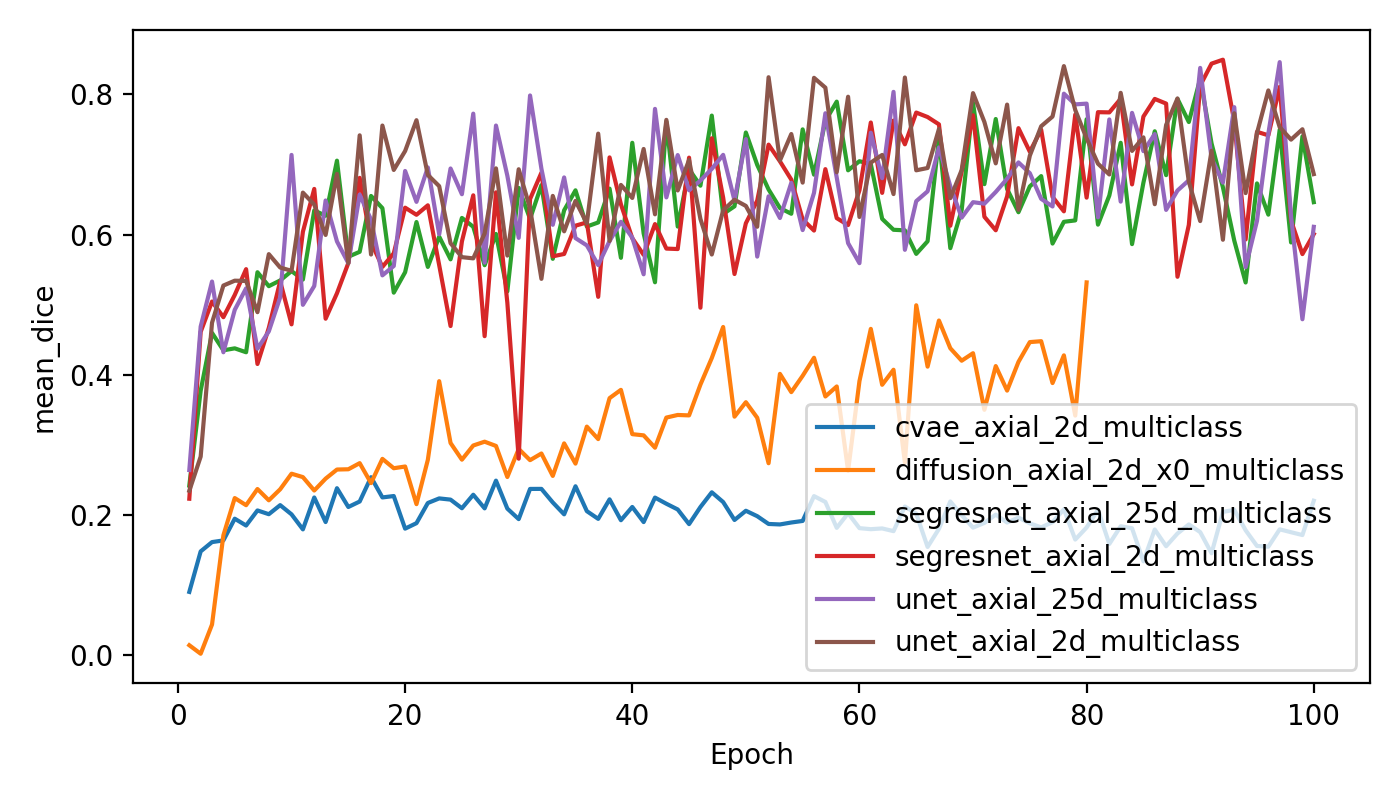
\includegraphics[width=\textwidth]{assets/axial_mean_dice.png}
      \sourcefoot{验证集 Mean Dice}
  \end{columns}
  \begin{alertblock}{观察}
    cVAE 收敛较早但测试泛化较弱；x0 diffusion 训练到后期仍有提升。2D diffusion 验证 Mean Dice 达到 0.532，2.5D diffusion 进一步达到 0.617。
  \end{alertblock}
\end{frame}

\begin{frame}{主实验结果}
  \begin{block}{KiTS23 axial test set}
    \centering
    \scriptsize
    \setlength{\tabcolsep}{3.2pt}
    \begin{tabular}{llrrrrr}
      \toprule
      模型 & 类型 & Mean & 肾脏 & 肿瘤 & 囊肿 & ms/img \\
      \midrule
      U-Net 2D & 判别式 & 0.570 & 0.912 & 0.623 & 0.177 & 2.57 \\
      SegResNet 2D & 判别式 & 0.572 & 0.914 & 0.621 & 0.181 & 4.46 \\
      U-Net 2.5D & 判别式 & \metricup{0.623} & 0.921 & 0.707 & 0.242 & 2.49 \\
      cVAE & 生成式 & 0.201 & 0.521 & 0.058 & 0.023 & 1.24 \\
      x0扩散 2D, 5步 & 生成式 & 0.434 & 0.820 & 0.449 & 0.032 & 67.43 \\
      x0扩散 2.5D, 5步 & 生成式 & \metricup{0.534} & 0.891 & 0.610 & 0.101 & 67.40 \\
      \bottomrule
    \end{tabular}
  \end{block}
  \begin{columns}[T]
    \column{0.48\textwidth}
      \begin{exampleblock}{生成式模型结果}
        x0 diffusion 明显优于 cVAE；加入相邻切片后，生成式模型从 0.434 提升到 0.534。
      \end{exampleblock}
    \column{0.48\textwidth}
      \begin{alertblock}{主要差距}
        2.5D diffusion 已接近 2D 判别式基线，但仍低于 2.5D U-Net；cyst 仍是最困难类别。
      \end{alertblock}
  \end{columns}
\end{frame}

\begin{frame}{采样步数消融}
  \begin{columns}[T]
    \column{0.46\textwidth}
      \begin{block}{x0 diffusion 测试集}
        \centering
        \setlength{\tabcolsep}{3.2pt}
        \begin{tabular}{rrrrr}
          \toprule
          输入 & 步数 & Mean Dice & Mean IoU & ms/img \\
          \midrule
          2D & 1  & 0.415 & 0.320 & 13.60 \\
          2D & 5  & 0.434 & 0.334 & 67.43 \\
          2.5D & 1  & \metricup{0.537} & \metricup{0.435} & 13.67 \\
          2.5D & 5  & 0.534 & 0.432 & 67.40 \\
          2.5D & 25 & 0.518 & 0.416 & 336.77 \\
          \bottomrule
        \end{tabular}
      \end{block}
    \column{0.50\textwidth}
      \begin{alertblock}{结论}
        在当前设置下，采样步数并非越多越好。2.5D 输入显著提升 Dice；1 步和 5 步结果接近，25 步没有继续提升。
      \end{alertblock}
      \begin{exampleblock}{解释}
        分割任务更关注语义区域是否正确，多步迭代可能在 tumor/cyst 小区域累积误差；相邻切片上下文比单纯增加步数更有效。
      \end{exampleblock}
  \end{columns}
\end{frame}

\begin{frame}{定性结果：稳定结构与失败模式}
  \begin{columns}[T]
    \column{0.50\textwidth}
      \centering
      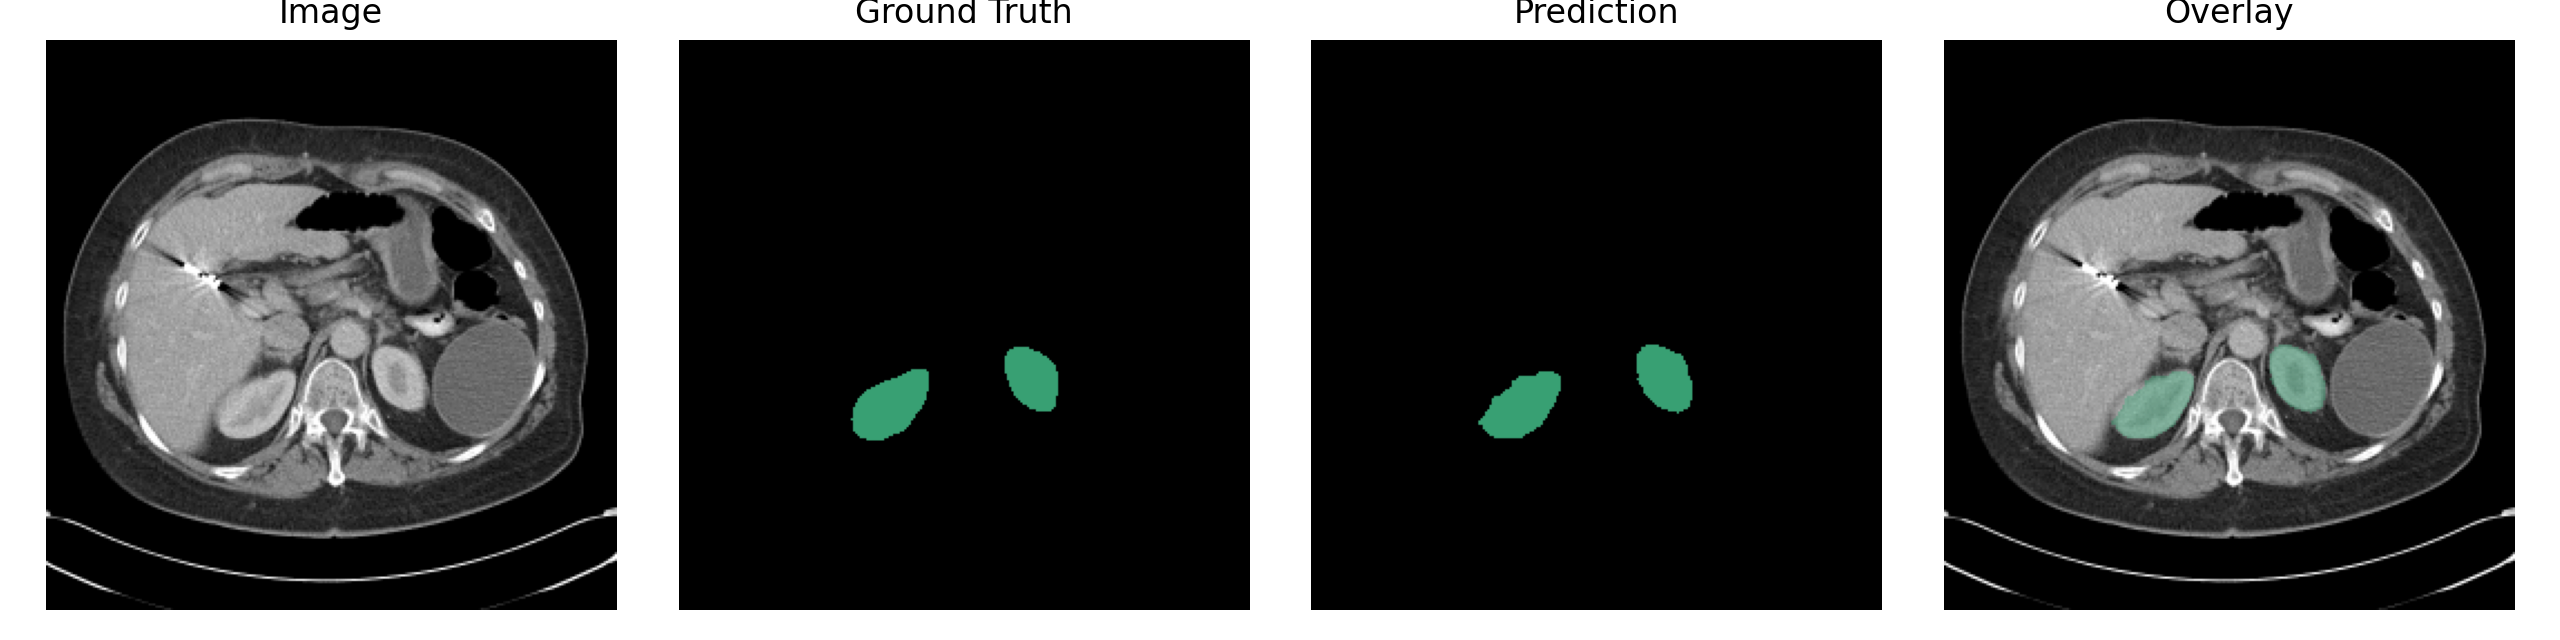
\includegraphics[width=\textwidth]{assets/axial_diffusion_case_success.png}
      \sourcefoot{稳定样例：双侧肾脏区域生成较完整。}
    \column{0.50\textwidth}
      \centering
      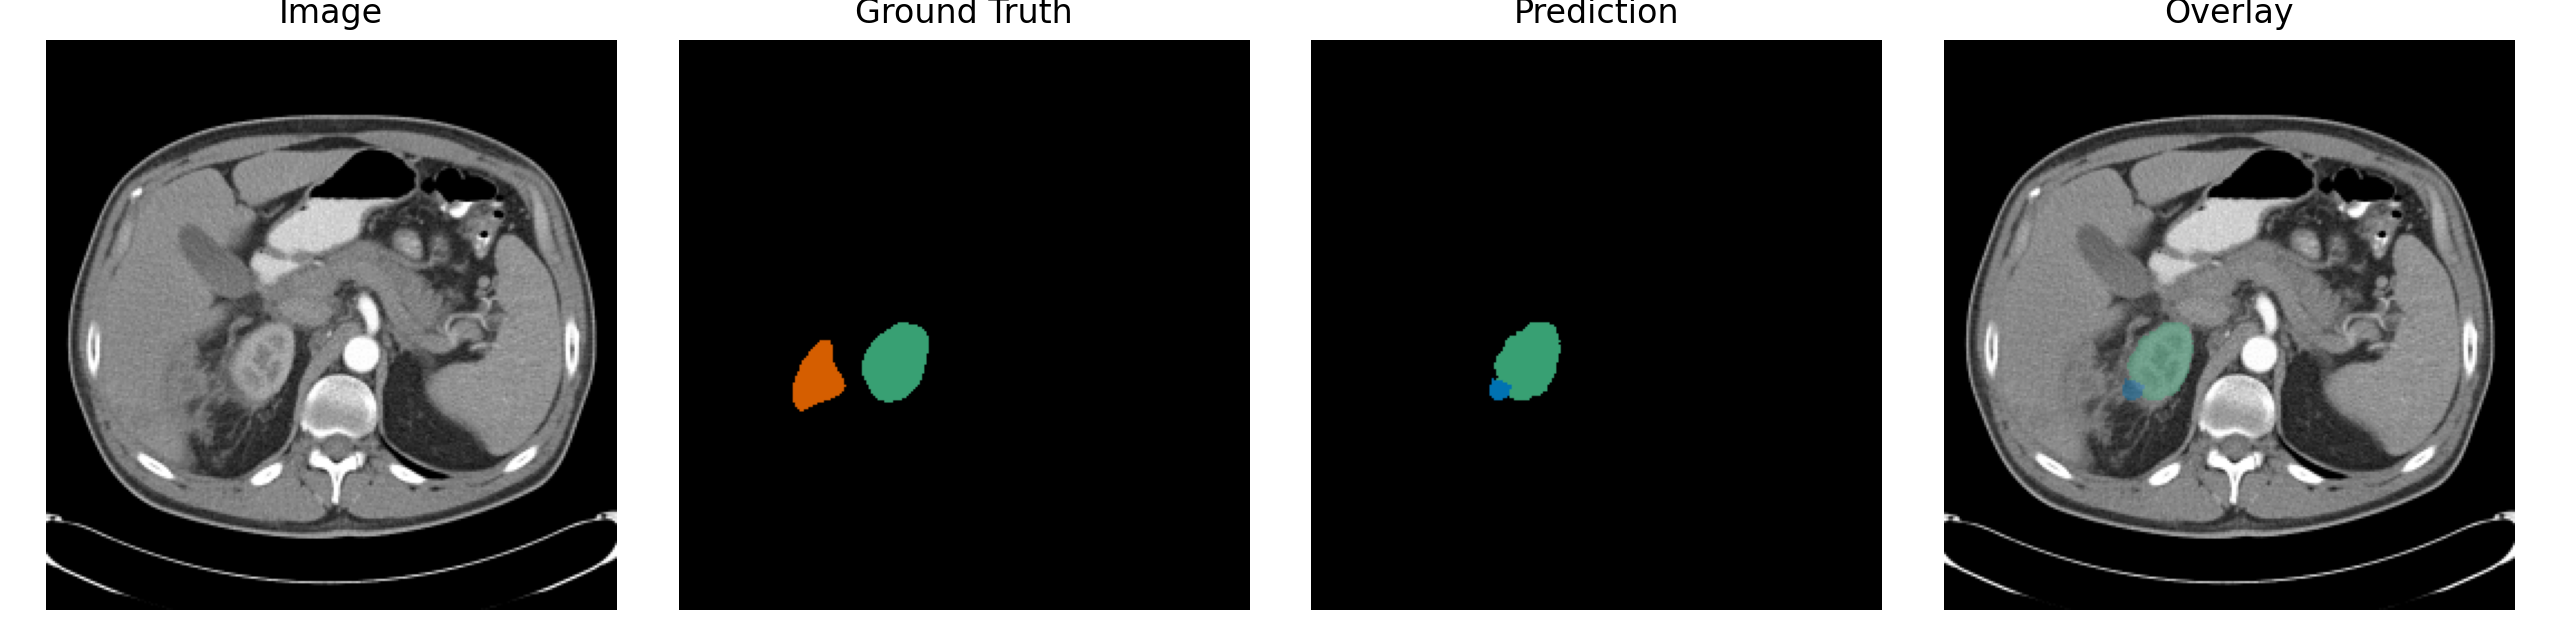
\includegraphics[width=\textwidth]{assets/axial_diffusion_case_failure.png}
      \sourcefoot{失败样例：小结构漏检或类别混淆。}
  \end{columns}
  \begin{alertblock}{读图要点}
    diffusion 可以生成合理 kidney 区域，但 tumor/cyst 边界和小目标容易漏检。这与定量结果中 kidney 高、cyst 低一致。
  \end{alertblock}
\end{frame}

\begin{frame}{生成过程与不确定性}
  \begin{columns}[T]
    \column{0.50\textwidth}
      \centering
      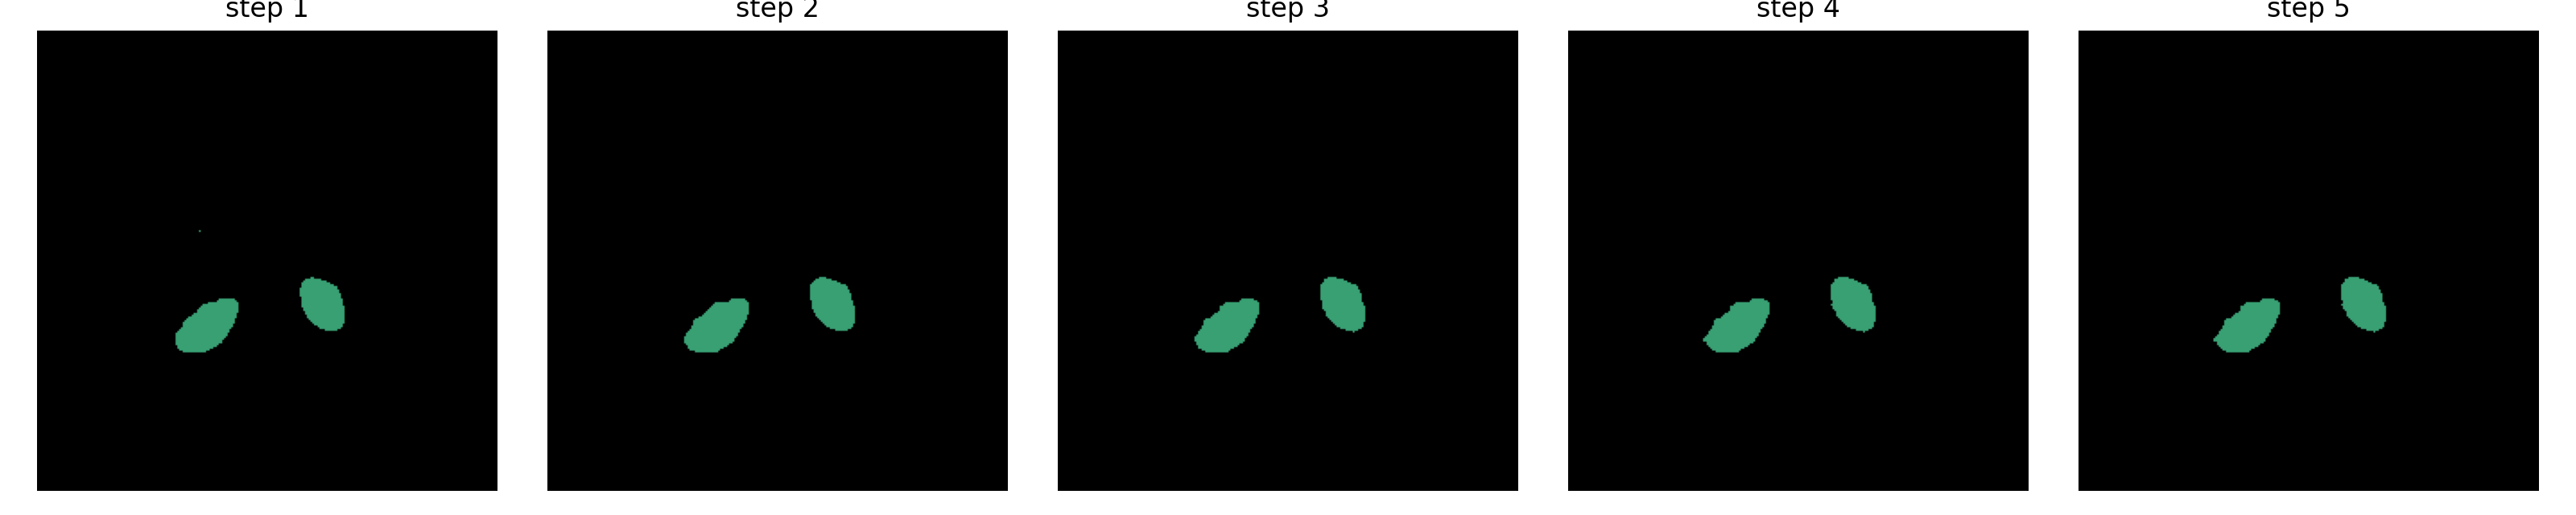
\includegraphics[width=\textwidth]{assets/axial_diffusion_denoising.png}
      \sourcefoot{去噪轨迹：由 noisy mask 逐步得到 clean mask。}
    \column{0.46\textwidth}
      \centering
      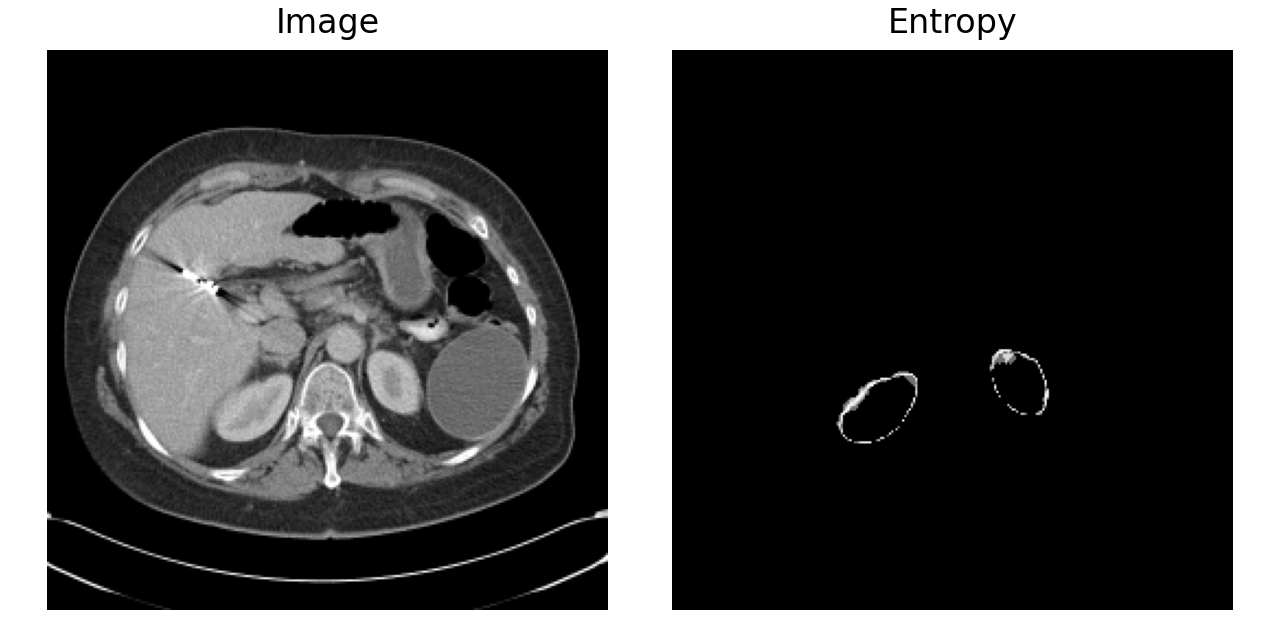
\includegraphics[width=\textwidth]{assets/axial_diffusion_uncertainty.png}
      \sourcefoot{不确定性图：由重复采样的预测熵得到。}
  \end{columns}
  \begin{exampleblock}{生成式模型的额外价值}
    与判别式模型相比，扩散模型可以展示生成过程，并通过重复采样给出边界和小病灶附近的不确定性提示。
  \end{exampleblock}
\end{frame}

\section{总结}

\begin{frame}{结论}
  \begin{columns}[T]
    \column{0.49\textwidth}
      \begin{exampleblock}{完成内容}
        \begin{itemize}
          \item 完成 KiTS23 四类分割数据处理和 patient-level split；
          \item 实现 U-Net、SegResNet、cVAE 和 x0 diffusion；
          \item 对比判别式与生成式模型，并分析采样步数和不确定性。
        \end{itemize}
      \end{exampleblock}
    \column{0.49\textwidth}
      \begin{alertblock}{核心结论}
        \begin{itemize}
          \item 2D x0 diffusion 的 Mean Dice 为 0.434，明显优于 cVAE 的 0.201；
          \item 2.5D x0 diffusion 进一步提升到 0.534，说明相邻切片上下文对生成式模型有效；
          \item 判别式模型仍然更强，2.5D U-Net 达到 0.623；
          \item 生成式模型的优势主要体现在生成过程和不确定性表达。
        \end{itemize}
      \end{alertblock}
  \end{columns}
\end{frame}

\begin{frame}{局限与后续方向}
  \begin{block}{主要局限}
    \begin{itemize}
      \item 2.5D diffusion 已明显优于 2D diffusion，但仍低于 2.5D U-Net；
      \item pixel-space mask diffusion 推理较慢，5 步约 67 ms/image；
      \item 当前只使用 100 例病例，未使用交叉验证、模型集成和强后处理。
    \end{itemize}
  \end{block}
  \begin{exampleblock}{可能提升方向}
    引入 2.5D/3D 条件编码、region-based label、前景区域裁剪、类别重加权 / focal loss，以及将 diffusion 用作判别式模型之后的 mask refinement。
  \end{exampleblock}
\end{frame}

\begin{frame}{参考资料与代码依据}
  \footnotesize
  \begin{block}{相关工作}
    \begin{itemize}
      \item Ronneberger et al., U-Net, MICCAI 2015
      \item Ho et al., Denoising Diffusion Probabilistic Models, NeurIPS 2020
      \item Song et al., Denoising Diffusion Implicit Models, ICLR 2021
      \item Wu et al., MedSegDiff / MedSegDiff-V2
      \item KiTS23 official repository and challenge reports
    \end{itemize}
  \end{block}
  \begin{block}{本地代码与结果}
    \begin{multicols}{2}
      \tiny
      \codepath{src/models/cvae_seg.py}\\
      \codepath{src/models/diffusion_unet.py}\\
      \codepath{src/diffusion/scheduler.py}\\
      \codepath{src/engine/train_diffusion.py}\\
      \codepath{results/tables/evaluation_main.csv}\\
      \codepath{results/tables/evaluation_axial_extended.csv}
    \end{multicols}
  \end{block}
\end{frame}

\begin{frame}{谢谢}
  \begin{center}
    \vspace{1em}
    {\Huge\color{ruc}\sffamily 谢谢}\\[1em]
  \end{center}
\end{frame}

\end{document}
